\documentclass[a4paper, 11pt]{article}
\usepackage[left = 2.5cm, right = 2.5cm , top = 1.5cm, bottom = 1.5cm]{geometry}
\usepackage{lipsum}
\usepackage[utf8]{inputenc}
\usepackage{indentfirst}
\usepackage{amsmath, amsfonts, amssymb,amsthm}
\usepackage{float}
\usepackage[pdftex]{graphicx}
\usepackage{booktabs}
\usepackage{graphicx}
\usepackage[portuguese]{babel}
\usepackage{multirow}
\usepackage{multicol}
\usepackage[T1]{fontenc}
\usepackage{enumitem}
\usepackage{titling}
\usepackage{cite}
\usepackage{url}
\usepackage{subfigure}
\usepackage[toc]{appendix}
\usepackage{listings}
\usepackage{array}
\usepackage{microtype}
\usepackage{mathpazo}
\newcommand{\subtitle}[1]{%
  \posttitle{%
    \par\end{center}
    \begin{center}\large#1\end{center}
    \vskip0.5em}%
}

\usepackage{xcolor}

\usepackage{hyperref}
\hypersetup{colorlinks=true,
	linkcolor=blue,
	urlcolor=blue,%black,
	citecolor=blue,
	pdfhighlight=/N
}


\title{\textbf{Osciladores acoplados}}
\subtitle{Relatório técnico apresentado ao professor Wesley Cota\\ como parte das exigências da disciplina Fis 492}
\author{Timóteo Fassoni e Airton Ferreira}


\begin{document}
\maketitle

\section{Introdução e motivação}


	Um sistema mecânico de grande interesse é o de osciladores acoplados. O exemplo mais simples consiste em dois pêndulos ligados por uma mola sujeitos a oscilar no plano vertical definido pelas suas posições de equilíbrio. Seja $d$ a distância entre os pêndulos (igual ao comprimento natural da mola, sem distender), $k$ a constante elástica da mola e considera-se que ambos sejam idênticos (mesma massa $m$ e comprimento $l$ da corda). Nessas circunstâncias, as equações de movimento são dadas, definindo $\omega_0^2=g/l$, por:
	\begin{equation}\label{eq :: equação do sistema}
	\begin{cases}
	m\ddot{x}_1 = - m\omega_0^2x_1 + k(x_2-x_1)\\
	m\ddot{x}_2 = - m\omega_0^2x_2 + k(x_1-x_2).
	\end{cases}
	\end{equation}
    A Figura \ref{figura :: pendulos acoplados} ilustra o problema dos dois pêndulos acoplados por uma mola.
    
    \begin{figure}[h!]
        \centering
        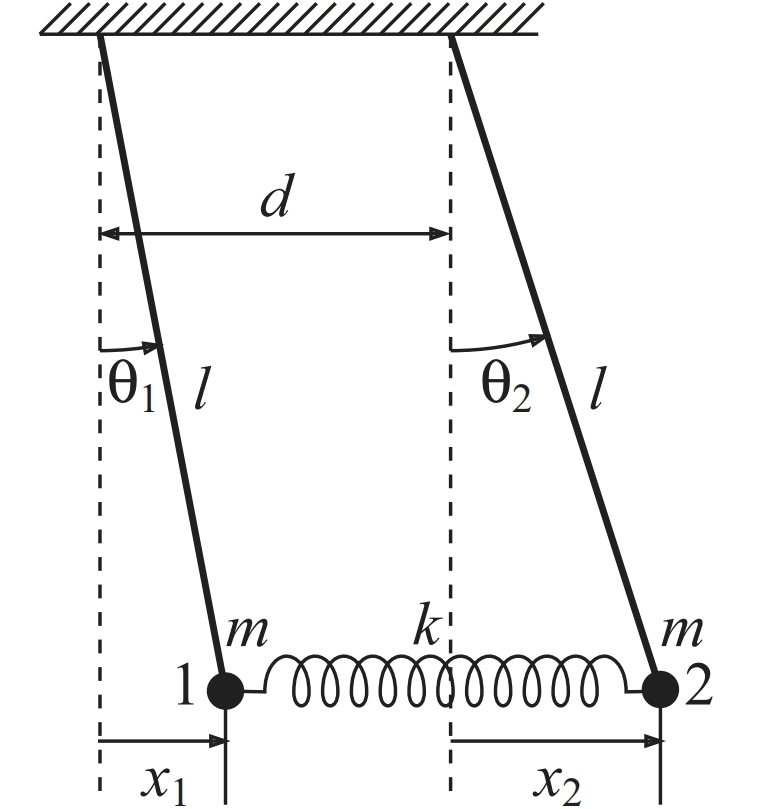
\includegraphics[width=0.3\linewidth]{pendulos_acoplados.jpg}
        \caption{Ilustração do problema dos dois pêndulos acoplados. Retirado de \cite{moyses_2}.
        \label{figura :: pendulos acoplados}}
    \end{figure}


	Para resolver o sistema, utiliza-se as coordenadas (modos) normais, um conjunto $\left\lbrace q_j\right\rbrace$ de coordenadas linearmente independentes dadas por combinações lineares do conjunto $\left\lbrace x_j\right\rbrace$ e que cada uma tem a solução complexa da forma\footnote{Uma constante de fase $\varphi_j$ pode ser acrescentada à dependência exponencial para ajuste de condições iniciais.}
	\begin{equation}
	\hat{q}_j = C_je^{\omega_jit},
	\end{equation}
onde $\omega_j$ é a frequência associada a cada modo normal $q_j$. Para o caso dos pêndulos acoplados, uma vez que as coordenadas normais têm soluções harmônicas, faz-se $x_1 = A_1e^{\omega it}$ e $x_2 = A_2e^{\omega it}$ para encontrar o conjunto de frequências normais, de modo que:
	\begin{equation}
	\begin{cases}
	-mA_1\omega^2e^{\omega it} = - mA_1\omega_0^2e^{\omega it} + k (A_2-A_1)e^{\omega it}\\
	-mA_2\omega^2e^{\omega it} = - mA_2\omega_0^2e^{\omega it} + k (A_1-A_2)e^{\omega it}.
	\end{cases}
	\end{equation}
Isto é,
	\begin{equation}
	\begin{cases}
		mA_1\omega^2 - mA_1\omega_0^2 + k (A_2-A_1) = 0 \\
		mA_2\omega^2 - mA_2\omega_0^2 + k (A_1-A_2) = 0
	\end{cases}
	\implies
	\begin{cases}
		\left( m(\omega^2-\omega_0^2) - k\right) A_1 + k A_2 = 0  \\
		kA_1 + \left( m(\omega^2-\omega_0^2) - k\right) A_2 = 0 
	\end{cases},
	\end{equation}
que, escrevendo na notação matricial, fica:
	\begin{equation}
	\left[\begin{matrix}
	\left( m(\omega^2-\omega_0^2) - k\right) & k \\
	k & \left( m(\omega^2-\omega_0^2) - k\right)
	\end{matrix}\right]
	\left(\begin{matrix}
	A_1\\
	A_2
	\end{matrix}\right)
	= 0,
	\end{equation}
de modo que as soluções não triviais são dadas por
	\begin{equation}
	\left|\begin{matrix}
	\left( m(\omega^2-\omega_0^2) - k\right) & k \\
	k & \left( m(\omega^2-\omega_0^2) - k\right)
	\end{matrix}\right|
	= 0 \implies \omega_1^2 = \omega_0^2 \hspace{0.2cm}\text{ e }\hspace{0.2cm} \omega_2^2 = \omega_0^2+2k/m,
	\end{equation}
que são as frequências de oscilação das coordenadas normais. Os autovetores $(A_1,A_2)$ associados a elas são $(1,1)$ e $(1,-1)$, de modo que as coordenadas normais podem ser escritas por:
	\begin{equation}
	q_1 = \dfrac{1}{2}(x_1+x_2) \hspace{0.7cm}\text{e}\hspace{0.7cm} 	q_2 = \dfrac{1}{2}(x_1 - x_2),
	\end{equation}
onde a constante $1/2$ é adicionada de tal forma a $q_1$ corresponder à coordenada do centro de massa.
$q_2$ é a posição de $x_1$ relativa à massa 2.

	Ou seja, no problema desses dois pêndulos acoplados, o centro de massa do sistema ($q_1$) e a posição de um em relação ao outro ($q_2$) executam um movimento harmônico simples, cada um com uma frequência $\omega_1$ e $\omega_2$. As coordenadas naturais do sistema, $x_1$ e $x_2$, podem ser obtidas pela transformação linear $x_1=q_1+q_2$ e $x_2 = q_1-q_2$. 

    \begin{figure}[h!]
        \centering
        \subfigure[Condições iniciais iguais]{
        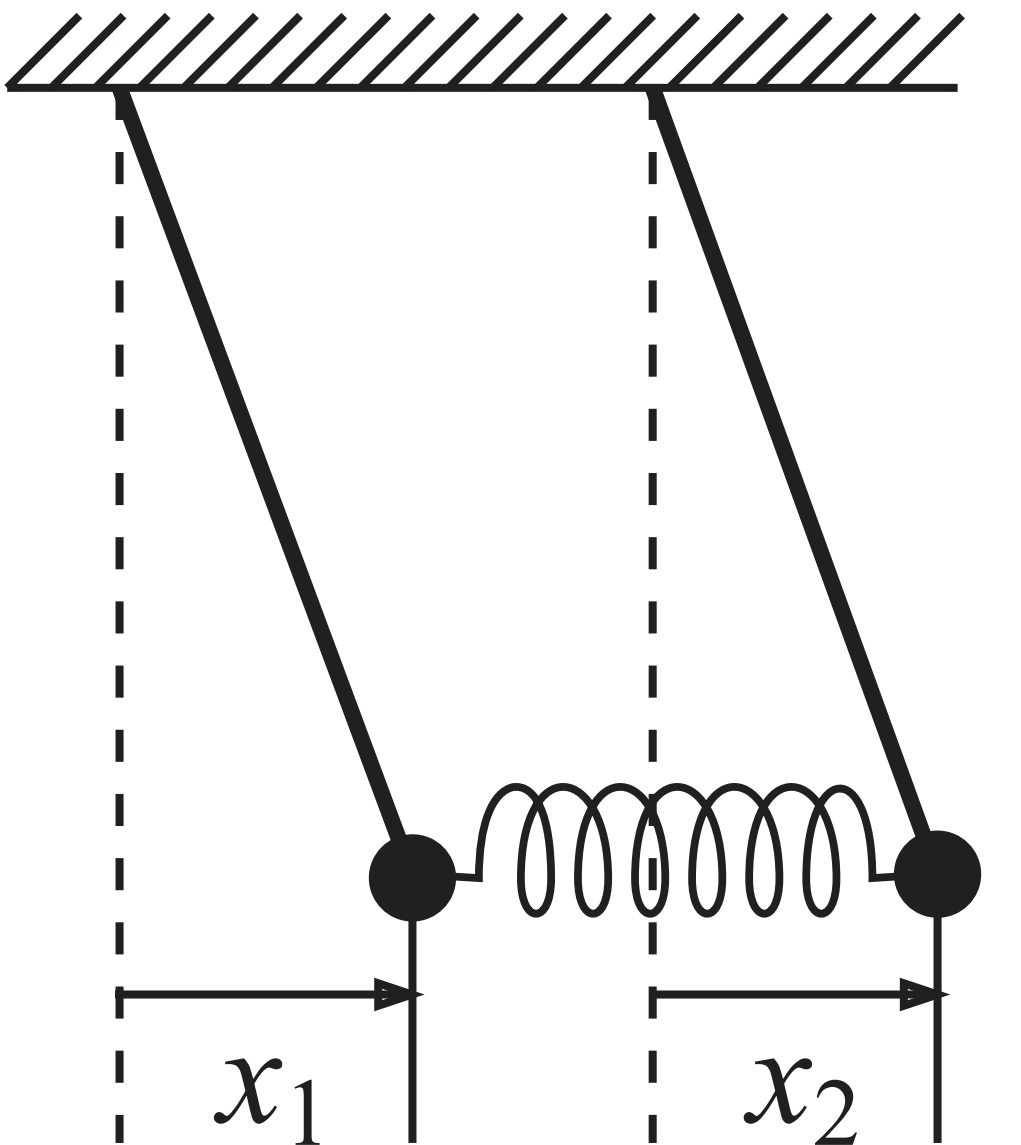
\includegraphics[height=0.3\linewidth]{condicoes_iguais.jpg}}
        \subfigure[Condições iniciais opostas]{
        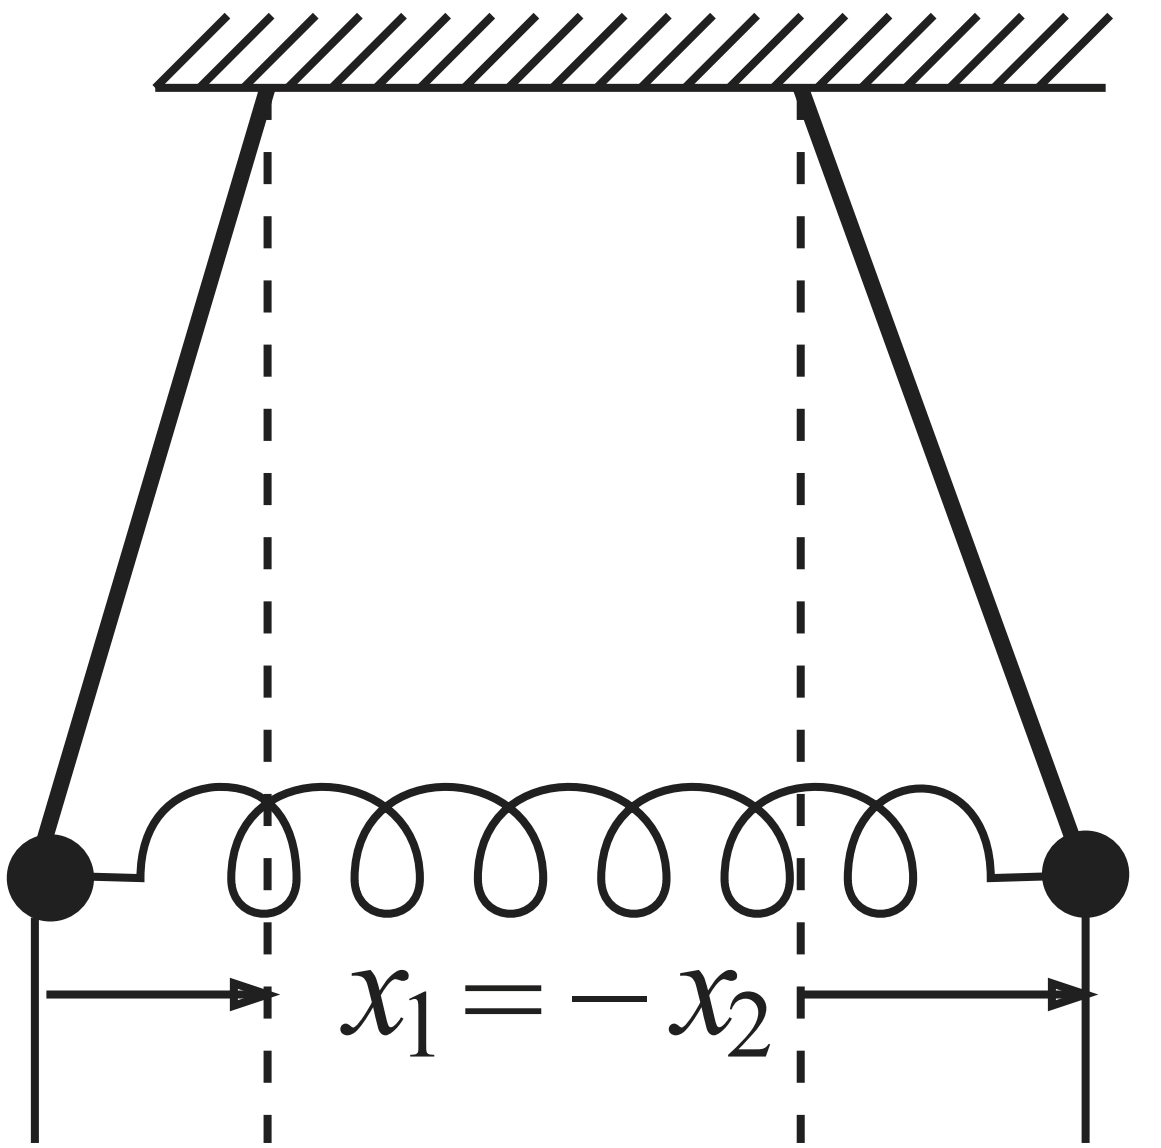
\includegraphics[height=0.3\linewidth]{condicoes_diferentes.jpg}}
        \caption{Condições inicias para demonstração da independência linear dos modos normais. Estes também são chamados de modo simétrico e modo anti-simétrico.
        \label{figura :: condições iniciais}}
    \end{figure}

    Este problema foi tratado para três condições inicias distintas. A primeira, de condições iniciais iguais, é definida por:
    \begin{equation}
    \begin{cases}
        x_1(t=0)=x_2(t=0)=x_0\\
        \dot{x}_1(t=0)=\dot{x}_2(t=0)=0.
    \end{cases}
    \end{equation}
    A segunda, de condições iniciais opostas, dada por:
    \begin{equation}
    \begin{cases}
        x_1(t=0)=-x_2(t=0)=x_0\\
        \dot{x}_1(t=0)=\dot{x}_2(t=0)=0.
    \end{cases}
    \end{equation}
    A Figura \ref{figura :: condições iniciais} mostra estas duas. Reescrevendo-as pelas coordenadas normais, ficam
    \begin{equation}
    \begin{cases}
        q_1(t=0)=x_0 \hspace{0.3cm}\text{e}\hspace{0.3cm} q_2(t=0)=0\\
        \dot{q}_1(t=0)=\dot{q}_2(t=0)=0,
    \end{cases}
    \end{equation}
    para o primeiro caso, e
    \begin{equation}
    \begin{cases}
        q_1(t=0)=0 \hspace{0.3cm}\text{e}\hspace{0.3cm} q_2(t=0)=x_0\\
        \dot{q}_1(t=0)=\dot{q}_2(t=0)=0,
    \end{cases}
    \end{equation}
    para a segunda. Assim, as condições inicias correspondem às soluções em que $(x_1,x_2)$ oscilam com a frequência de cada um dos modos normais (isto é, são, justamente, os autovetores comentados anteriormente) e podem ser utilizadas para mostrar a independência linear dos modos. A terceira, corresponde a:
    \begin{equation}
    \begin{cases}
        x_1(t=0)=x_1^0 \hspace{0.3cm}\text{e}\hspace{0.3cm} x_2(t=0)=x_2^0\\
        \dot{x}_1(t=0)=\dot{x}_1^0 \hspace{0.3cm}\text{e}\hspace{0.3cm} \dot{x}_2(t=0)=0,
    \end{cases}
    \end{equation}
    utilizada para ver o fenômeno de batimentos (de transmissão de energia de um para o outro pêndulo) e as diferenças entre as soluções para as coordenadas naturais e normais, bem como o espaço de fase do sistema.

    A teoria dos osciladores acoplados é muito útil para vários outros fenômenos. Por exemplo, o modelo de Debye para sólidos é baseado nessa ideia. A própria solução de onda para uma corda pode ser construída tratando como um conjunto de $N$ osciladores acoplados e fazendo $N\to\infty$. A ideia inicial é implementar a solução numérica com o método de Runge-Kutta de quarta ordem para integração numérica da Eq. \eqref{eq :: equação do sistema} e, posteriormente, implementar para o caso de $N$ osciladores para a corda -- a Figura \ref{figura :: modos normais para quatro osciladores} mostra os modos normais para $N=4$.

    \begin{figure}[h!]
        \centering
        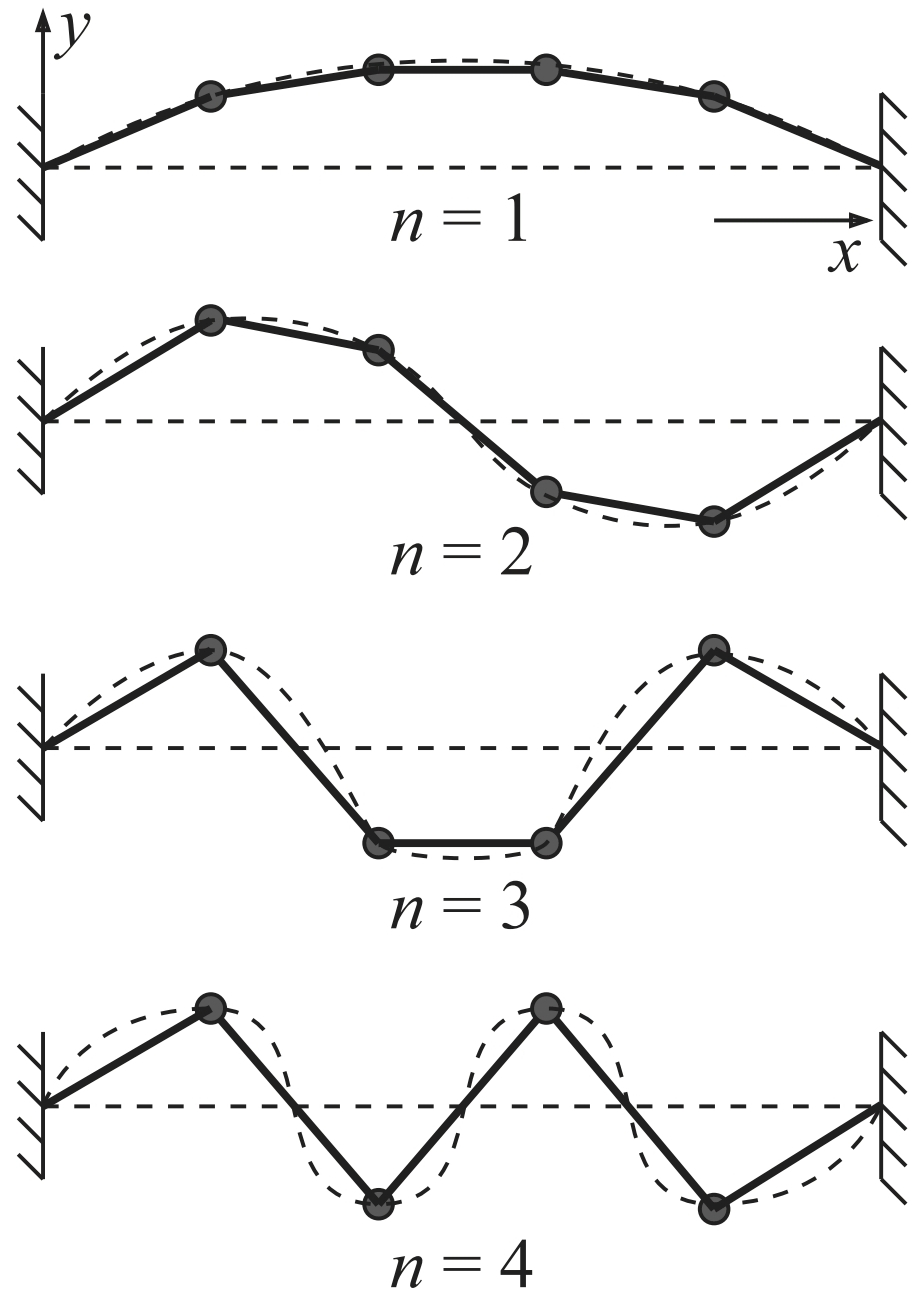
\includegraphics[width=0.6\linewidth]{modos_normais_para_quatro_osciladores.jpg}
        \caption{Modos normais para quatro osciladores acoplados numa corda.
        \label{figura :: modos normais para quatro osciladores}}
    \end{figure}

\newpage
\section{ Implementação }

    O programa foi desenvolvido em Fortran, utilizando o método de Runge-Kutta de quarta ordem (RK4) para a integração numérica das equações diferenciais do sistema, foi escolhido devido à sua precisão e estabilidade em simulações numéricas de sistemas dinâmicos.
    
    A simulação foi dividida em vários arquivos de programas, sendo a parte de fortran composta pelo programa principal \texttt{osc\_acopladas\_n.f90} e módulo \texttt{mod\_runge\_kutta.f90}, já a parte de análise gráfica foi desenvolvida em python, o qual e composto por \texttt{graph\_2\_pendulos.py} e \texttt{graph\_n\_pendulos.py} fazendo uso assim das bibliotecas \textit{numpy} e \textit{matplotlib}. A estrutura básica consiste nos seguintes componentes:

\begin{itemize}

    \item \textbf{Programa principal (\texttt{osc\_acopladas\_n})}: Configura os parâmetros iniciais, como número de pêndulos ($N$), as condições iniciais e as constantes físicas do sistema, conforme descrito anteriormente. Em seguida, chama o módulo \texttt{runge\_kutta} que vai fazer a integração numérica das equações diferenciais do sistema para péndulos acoplados. O código inclui uma interface que solicita ao usuário o número de pêndulos e a condição inicial a ser escolhida. Após as escolhas serem feitas, o programa termina de simular gerando os resultados, que são armazenados em arquivos de saída no formato \texttt{.dat}. Mais informações são descrita no arquivo \texttt{osc\_acopladas\_n.f90}.

    \item \textbf{Função auxiliar (\texttt{derivada\_z})}: Inclue as equações diferenciais acopladas (\ref{eq::pendulos_acoplados}), adaptadas para o cálculo de  $N$. É esta parte do código que pode ser substituída, pois, possui a flexibilidade de ser adaptada para outros sistemas descritos por EDOs, desde que possam ser reduzidos a sistemas de primeira ordem.

    \item \textbf{Módulo (\texttt{runge\_kutta})}: O módulo é composto pela função principal, \texttt{rk4\_multi}, responsável por calcular a evolução do sistema a cada passo de tempo, utilizando os coeficientes intermediários (\(k_1, k_2, k_3, k_4\)) para estimar o próximo estado do sistema. A função de derivadas, fornecida pelo usuário, define as taxas de variação das variáveis, e a solução numérica é obtida pela combinação ponderada desses coeficientes. Aqui destaca-se a importância da criação do módulo, pois ele torna o desenvolvimento mais flexível, permitindo fácil adaptação a diferentes sistemas dinâmicos e necessidades específicas de modelagem.
\end{itemize}

\subsection{Método de Runge-Kutta}

As equações diferenciais (\ref{eq::pendulos_acoplados}) foram reformuladas em termos de um sistema de primeira ordem. Seja $\mathbf{z}$ o vetor de estado, composto pelas coordenadas e suas derivadas, temos:

\begin{equation}
\mathbf{z} = \begin{bmatrix} x_1 \\ \dot{x}_1 \\ x_2 \\ \dot{x}_2 \end{bmatrix},
\end{equation}
com as equações diferenciais dadas por:
\begin{equation}
\begin{cases}
\dot{x}_1 = \dot{z}_2, \\
\ddot{x}_1 = -\omega_0^2 x_1 + \frac{k}{m}(x_2 - x_1), \\
\dot{x}_2 = \dot{z}_4, \\
\ddot{x}_2 = -\omega_0^2 x_2 + \frac{k}{m}(x_1 - x_2).
\end{cases}
\end{equation}

Essas equações são resolvidas iterativamente, atualizando o vetor $\mathbf{z}$ a cada passo de tempo $\Delta t=h$.

\subsection{Saída e Visualização dos Resultados}

Os resultados da simulação são gravados em arquivos de texto, permitindo sua posterior análise gráfica com ferramentas como o \textit{Matplotlib} no Python. A saída inclui:
\begin{itemize}
    \item Coordenadas naturais ($x_1, x_2$) e normais ($q_1, q_2$) ao longo do tempo.
    \item Perfis do espaço de fase para as coordenadas naturais e normais.
    \item Distribuição de energia entre as massas ao longo do tempo.
\end{itemize}

O código está estruturado para ser escalável, permitindo simular sistemas com qualquer número $N$ de pêndulos. A próxima etapa consiste em estender a análise para o caso de $N > 2$, explorando os modos normais de sistemas mais complexos.

\newpage
\section{ Resultados }

    A análise gráfica dos resultados foi feita no Python, com auxílio do pacote Matplotlib. Todos os dados foram normalizados e são dados em termos de unidades arbitrárias.
    
    \begin{figure}[h!]
        \centering
        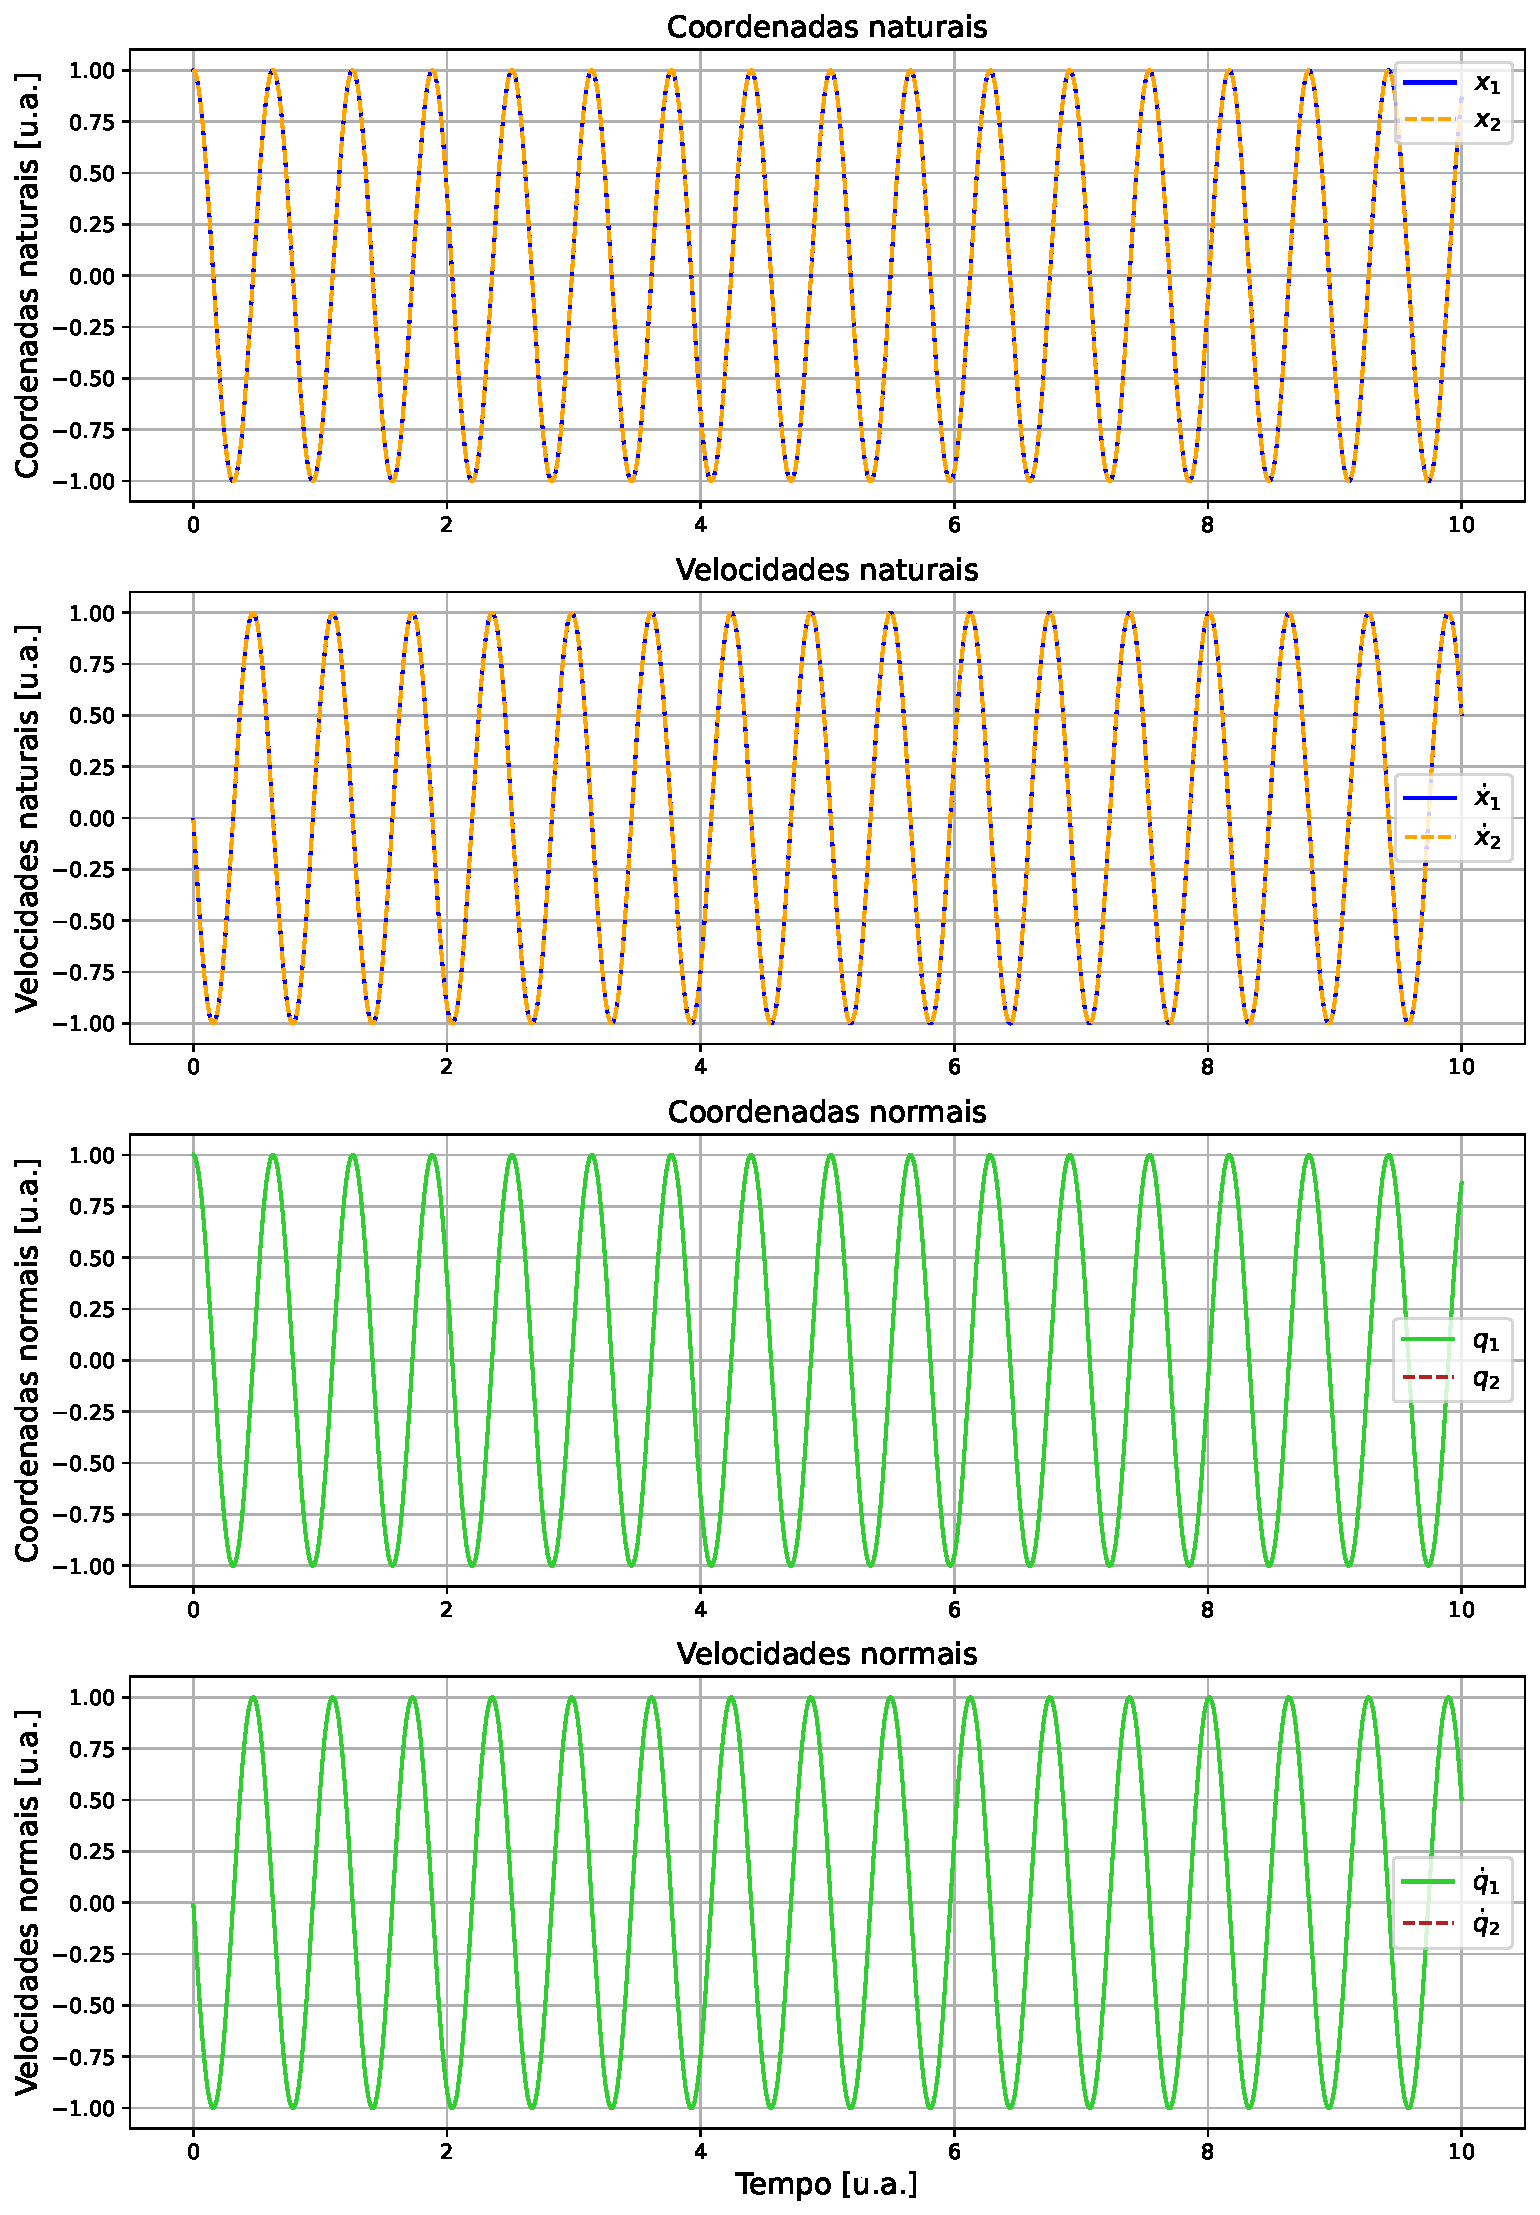
\includegraphics[width=1\linewidth]{graph_coordenadas_iguais.pdf}
        \caption{ Conjuntos de coordenadas $(x_1(t),x_2(t))$ e $(q_1(t),q_2(t))$ do sistema para condições iniciais iguais.
        \label{figura :: coordenadas condições iguais}}
    \end{figure}


    
    
    \begin{figure}[h!]
        \centering
        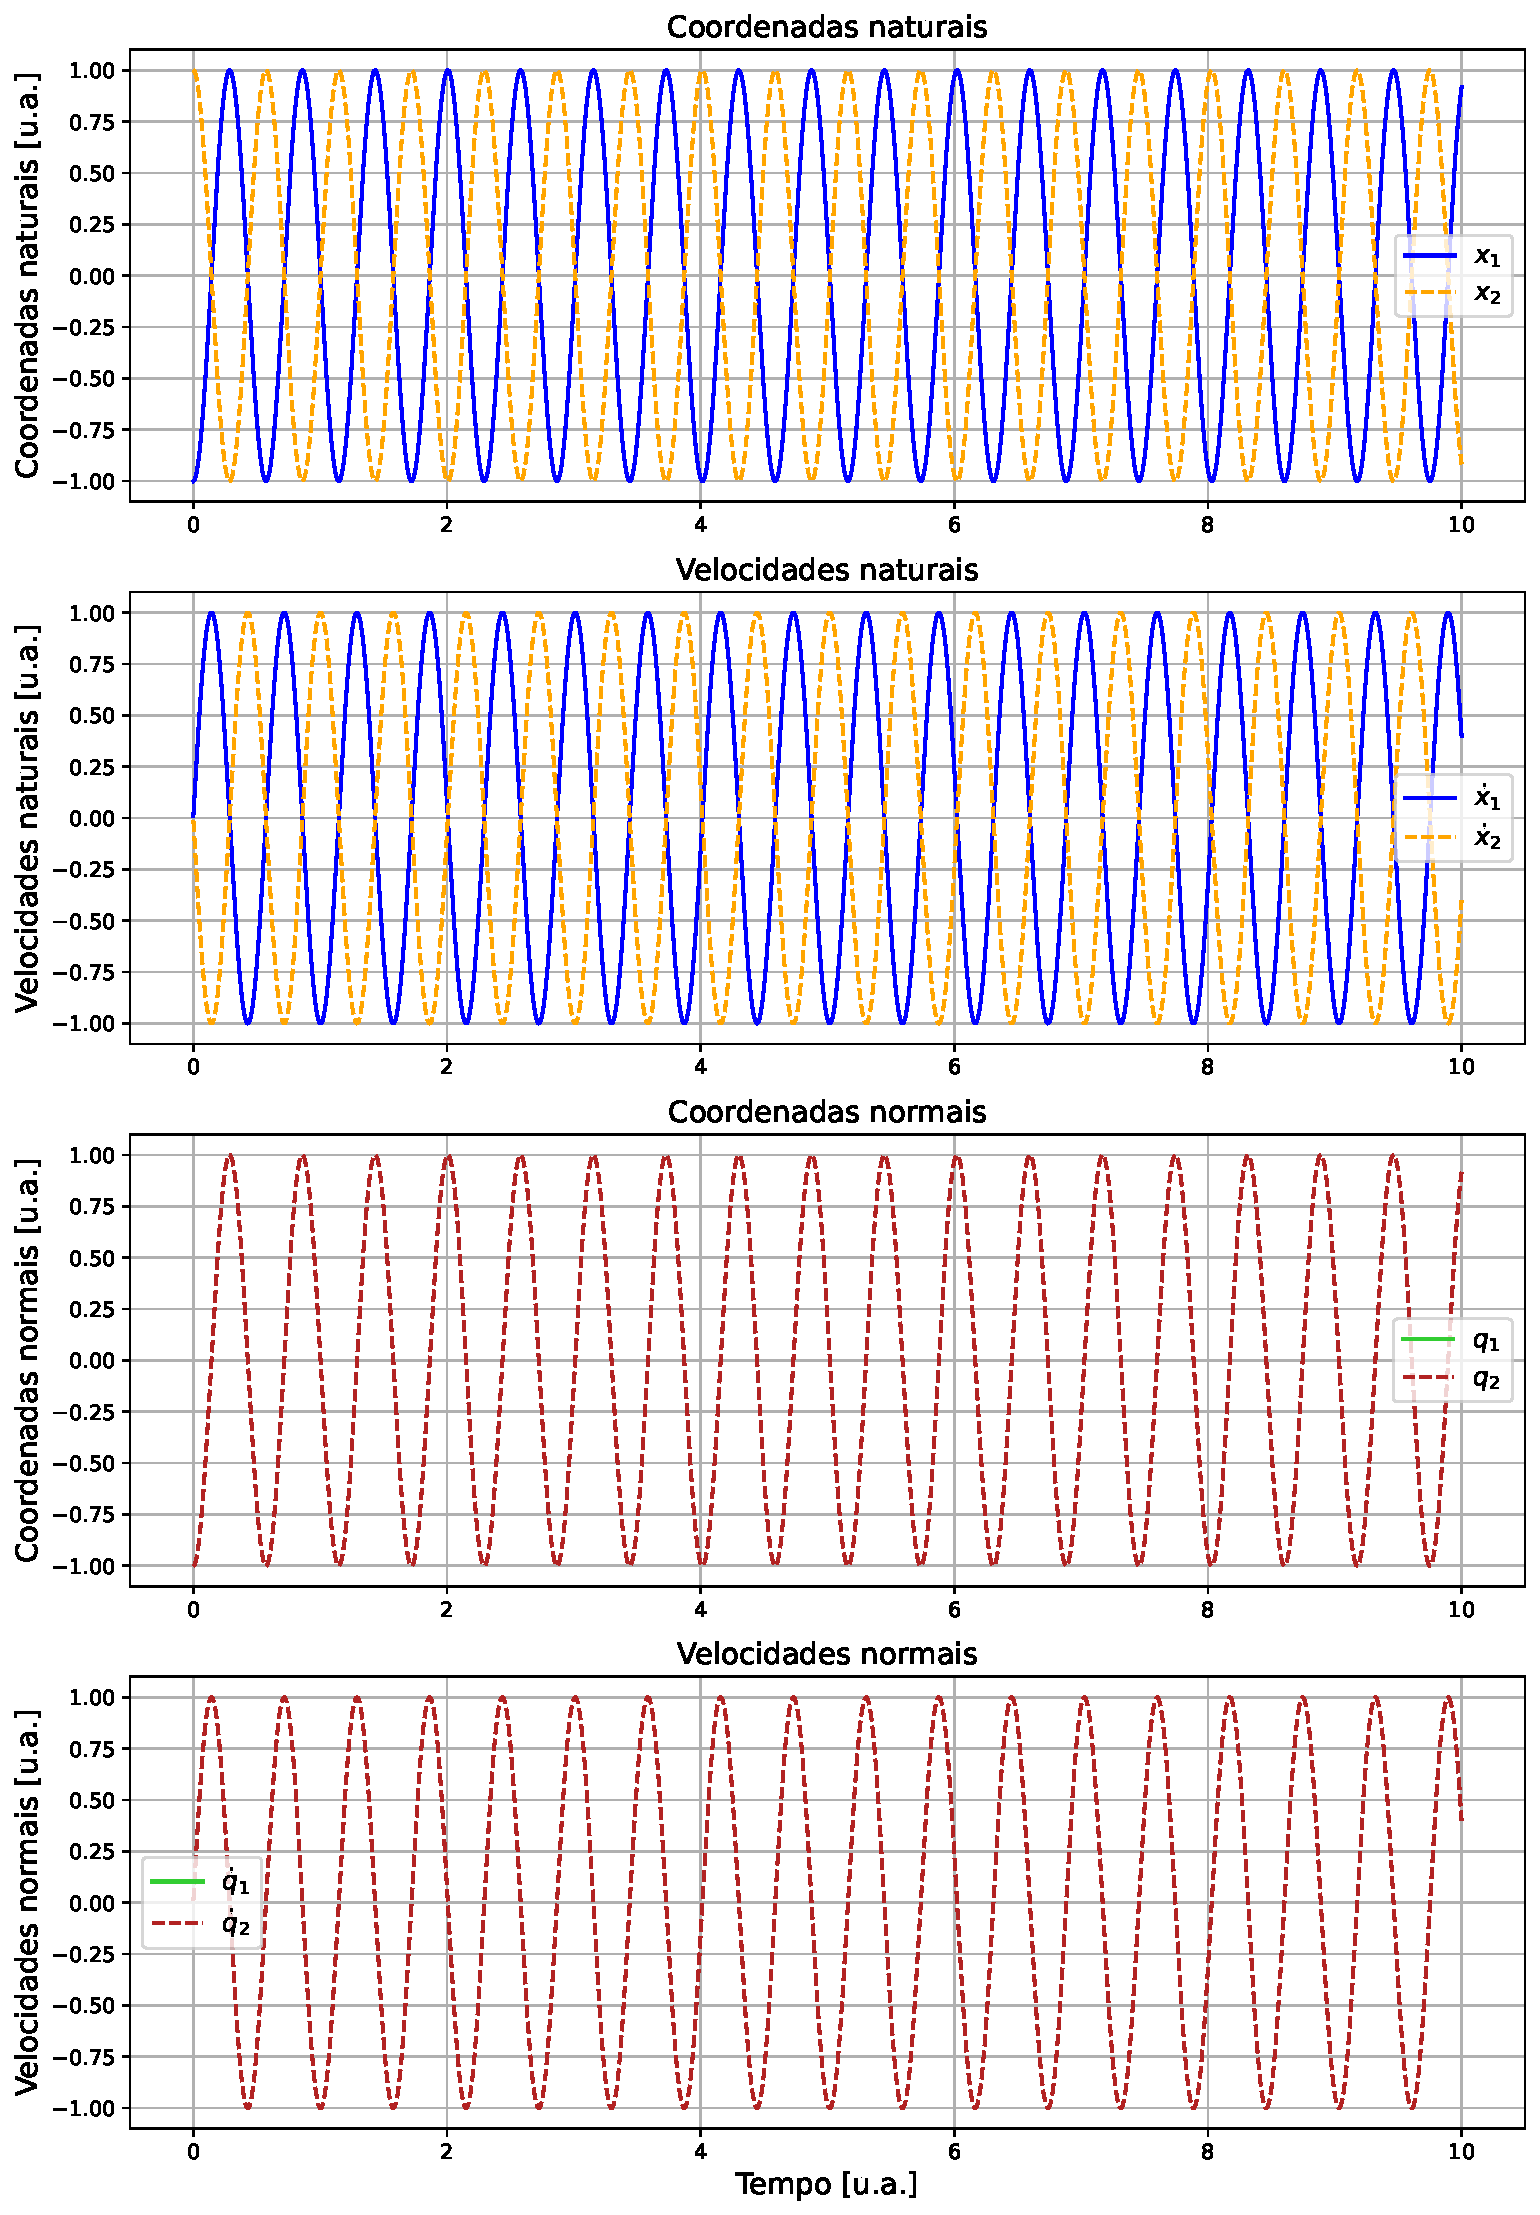
\includegraphics[width=1\linewidth]{graph_coordenadas_opostas.pdf}
        \caption{Conjuntos de coordenadas $(x_1(t),x_2(t))$ e $(q_1(t),q_2(t))$ do sistema para condições iniciais opostas.
        \label{figura :: coordenadas condições opostas}}
    \end{figure}

    As Figuras \ref{figura :: coordenadas condições iguais} e \ref{figura :: coordenadas condições opostas} mostram os resultados para as primeiras condições inicias. De fato, elas mostram que as coordenadas naturais oscilam harmonicamente de acordo com a coordenada normal que não é nula pelas condições inicias. Isso mostra que o conjunto $(q_1,q_2)$ é linearmente independente, uma vez que há soluções em que uma é autovetor do problema e a outra é identicamente nula. Estas soluções são os modos simétrico e anti-simétrico, respectivamente, como comentado.

    Para o terceiro caso, com as condições iniciais diferentes, as soluções para $(x_1,x_2)$ não são harmônicas. Os perfis dos dois espaços de fase -- isto é, os espaços definidos pelas coordenadas $(x_1,x_2,\dot{x}_1,\dot{x}_2)$ e $(q_1,q_2,\dot{q}_1,\dot{q}_2)$ -- dados pelos gráficos da velocidade com sua respectiva coordenada espacial mostram isso. Para o movimento harmônico, estes perfis são de elipses, o que é observado para os modos, enquanto as coordenadas naturais têm o perfil diferente (no geral, são dados pela família das curvas de Lissajous \cite{torton_marion}).

    \begin{figure}[h!]
        \centering
        \includegraphics[width=1\linewidth]{graph_espaços_de_fase.pdf}
        \caption{Perfis dos espaços de fase para cada coordenada. Para os modos, observa-se elipses, de acordo com o esperado para o movimento harmônico. Para as coordenadas naturais, observa-se padrões diferentes. A variação do raio das curvas (distância até a origem) é causada pela variação da energia em cada pêndulo dada pelo fenômeno de batimentos (ver Figura \ref{figura :: energia}).
        \label{figura :: espaços de fase}}
    \end{figure}

    \begin{figure}[h!]
        \centering
        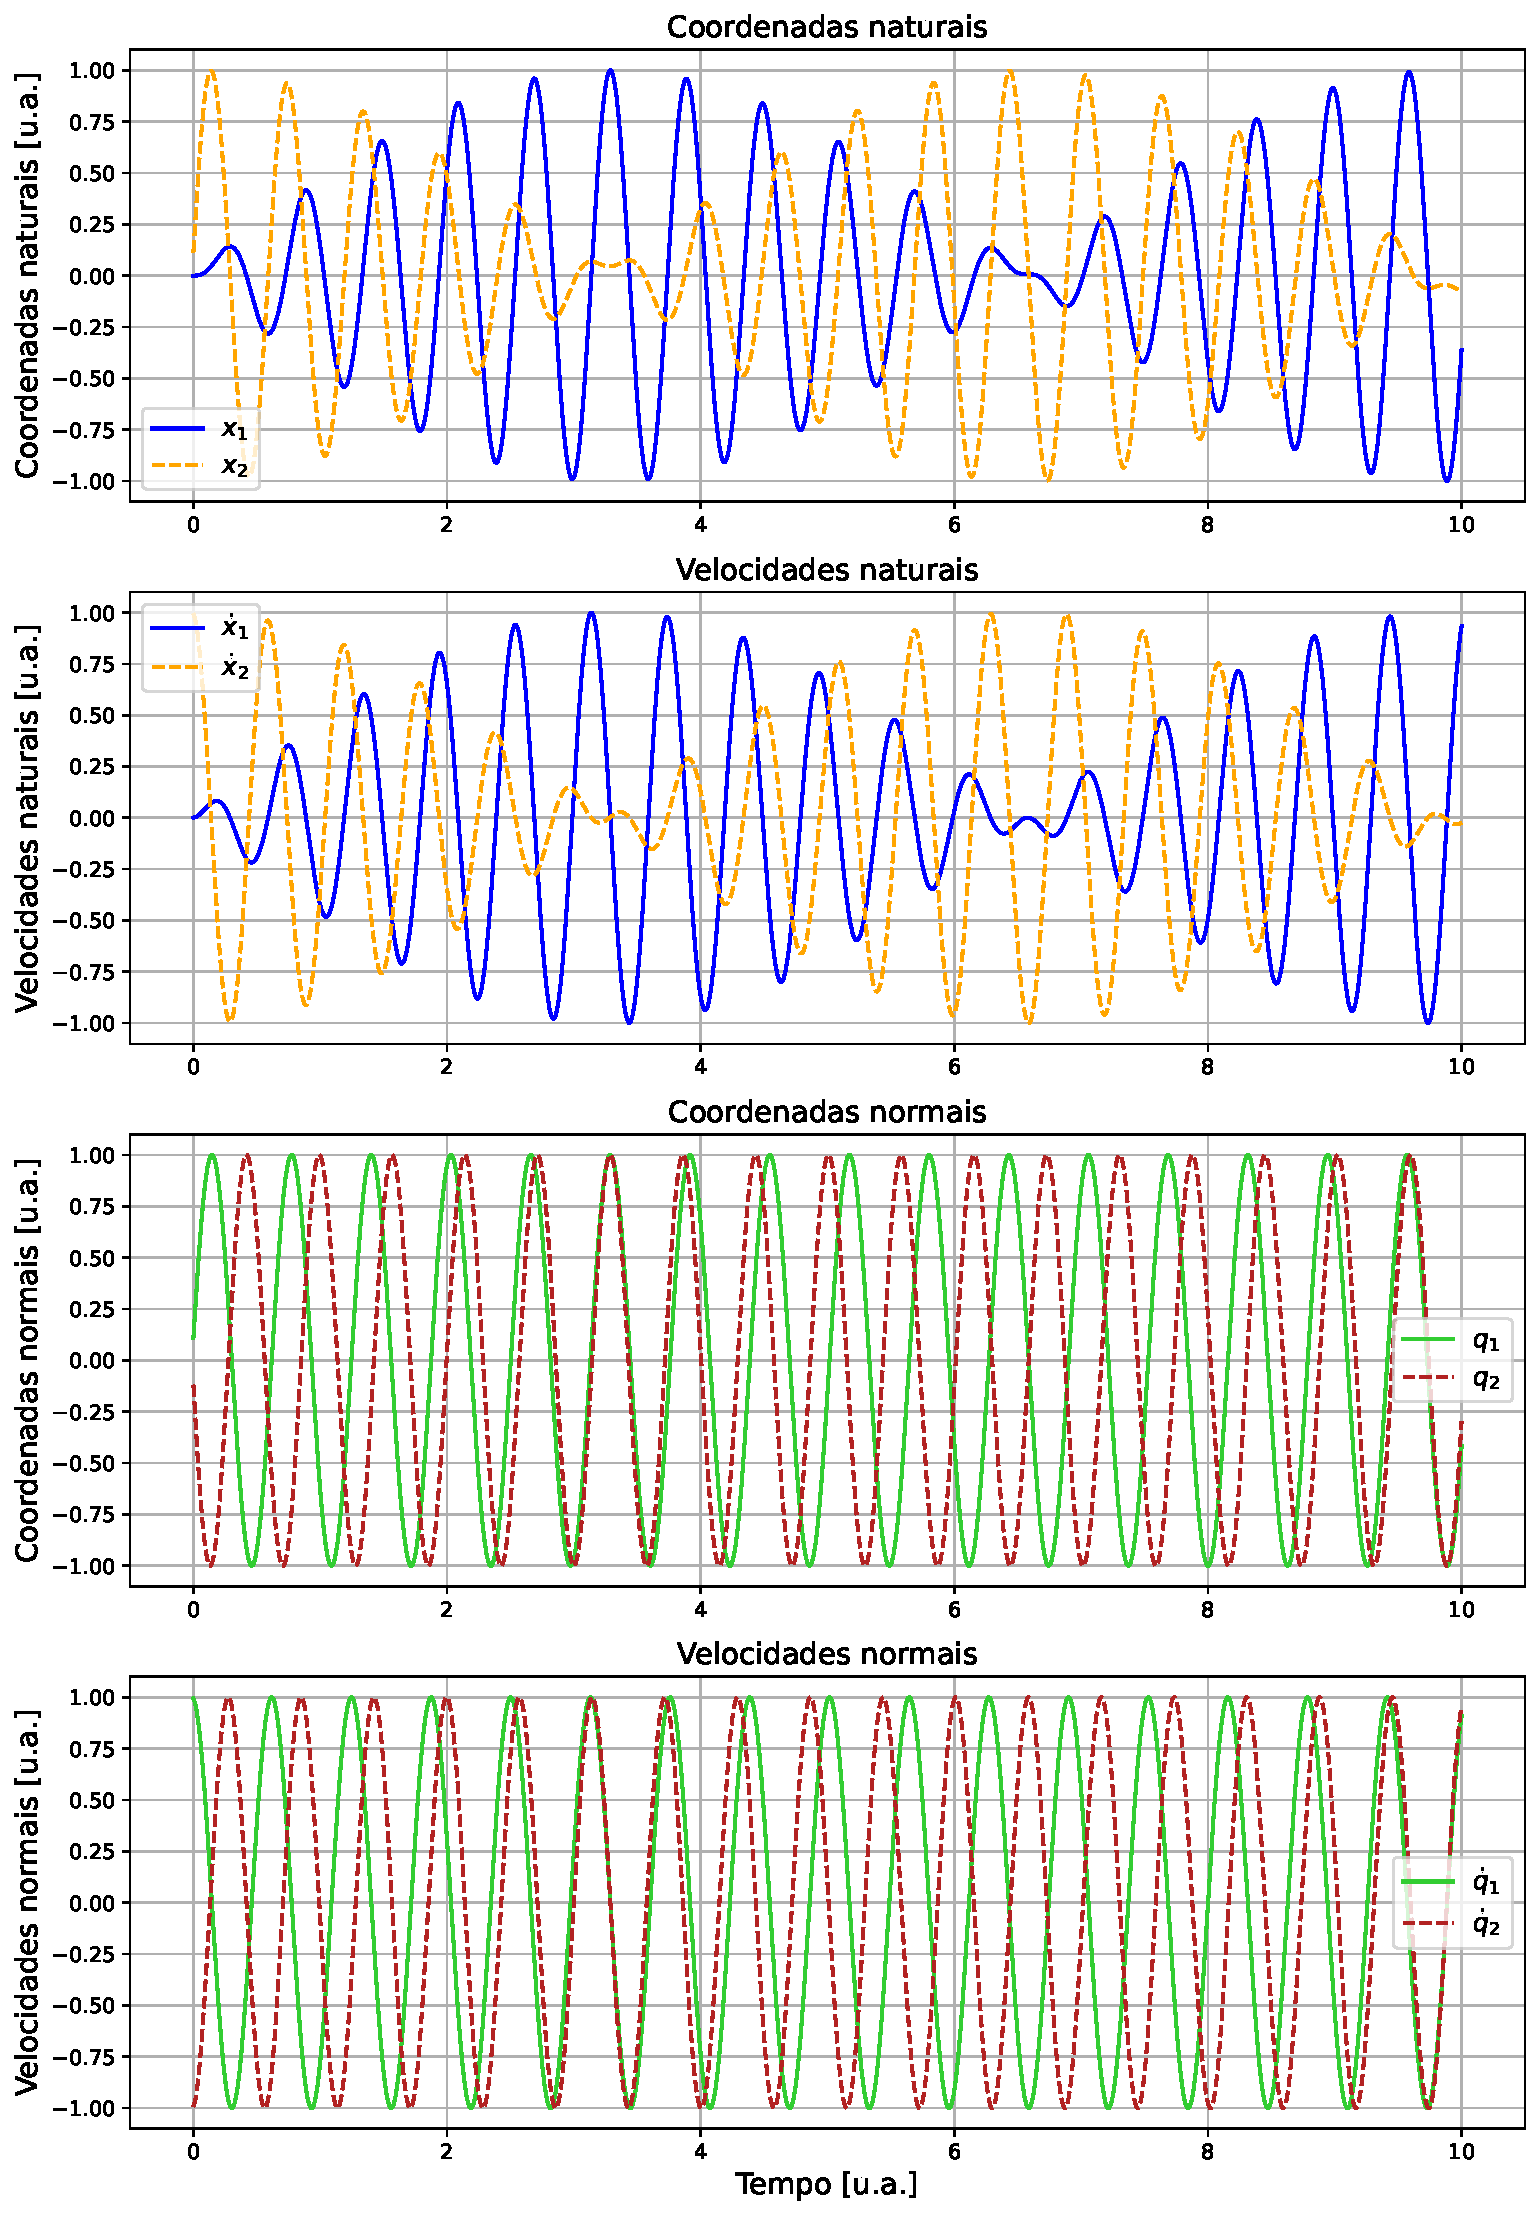
\includegraphics[width=1\linewidth]{graph_coordenadas_diferentes.pdf}
        \caption{Conjuntos de coordenadas $(x_1(t),x_2(t))$ e $(q_1(t),q_2(t))$ do sistema para condições diferentes.
        \label{figura :: coordenadas condições diferentes}}
    \end{figure}

    A Figura \ref{figura :: coordenadas condições diferentes} mostra as soluções para cada conjunto de coordenada para a terceira condição inicial. As coordenadas $(q_1,q_2)$, apesar do movimento harmônico, não se encontram em fase e têm frequências diferentes (como esperado). 

    Para as coordenadas $(x_1,x_2)$ observa-se o fenômeno de batimentos: um dos pêndulos começa a oscilar, e, pela interação da mola que os liga, a sua energia é transferida para o outro pêndulo, até quase parar e o outro oscilar com amplitude máxima. Depois, a energia é transferida novamente para o primeiro. Daí o fenômenos de batimentos. A Figura \ref{figura :: energia} mostra como a energia do sistema é distribuída entre os pêndulos, mostrando a sua conservação e a transmissão de energia de um para outro pêndulo: quando a de um é máxima, a do outro é mínima.

    Este fenômeno de batimentos é extremamente importante para todos os modelos onde aparecem as oscilações acopladas e as oscilações forçadas (por exemplo em circuitos elétricos) e está conectado, também, ao fenômeno de ressonância. É uma consequência clara da superposição e interferência de movimentos harmônicos (e, dessa forma, de ondas). 

    \begin{figure}[h!]
        \centering
        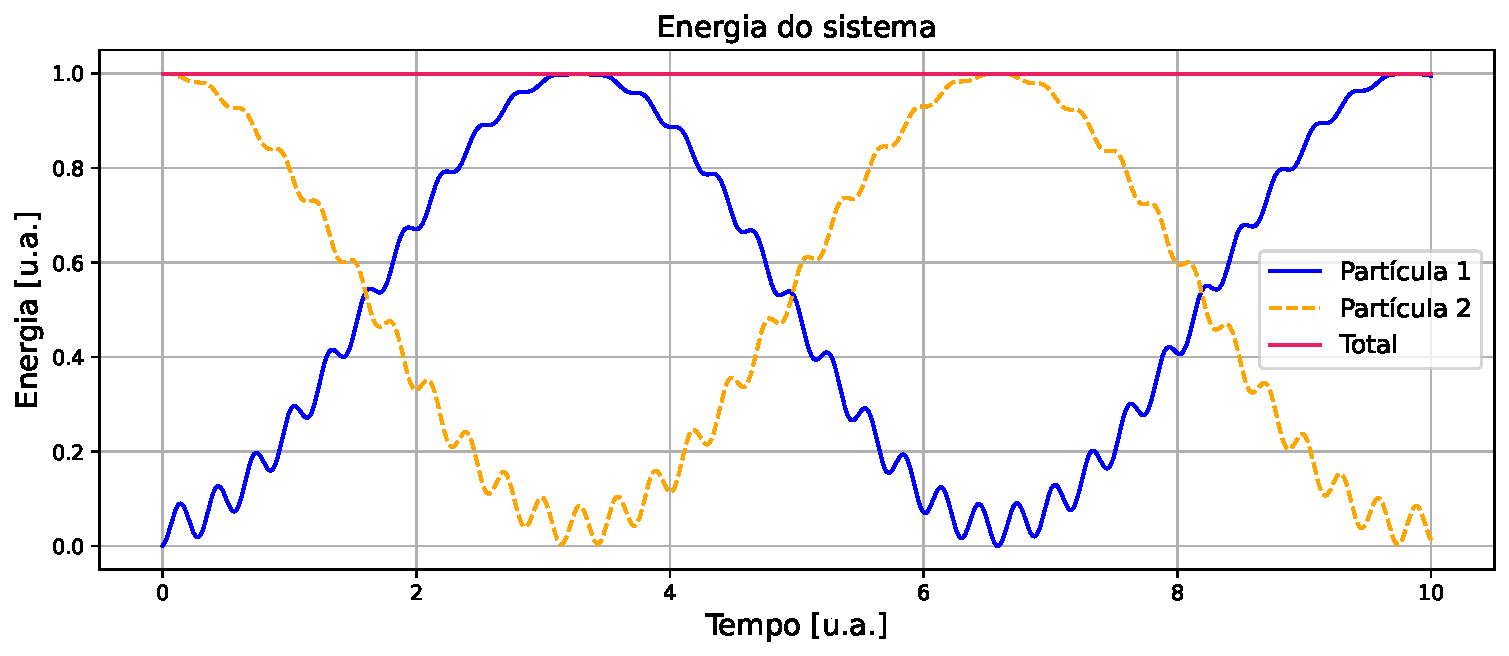
\includegraphics[width=1\linewidth]{graph_energia.pdf}
        \caption{Distribuição da energia do sistema entre as duas massas, mostrando o fenômeno de batimentos.
        \label{figura :: energia}}
    \end{figure}

    \begin{figure}[h!]
        \centering
        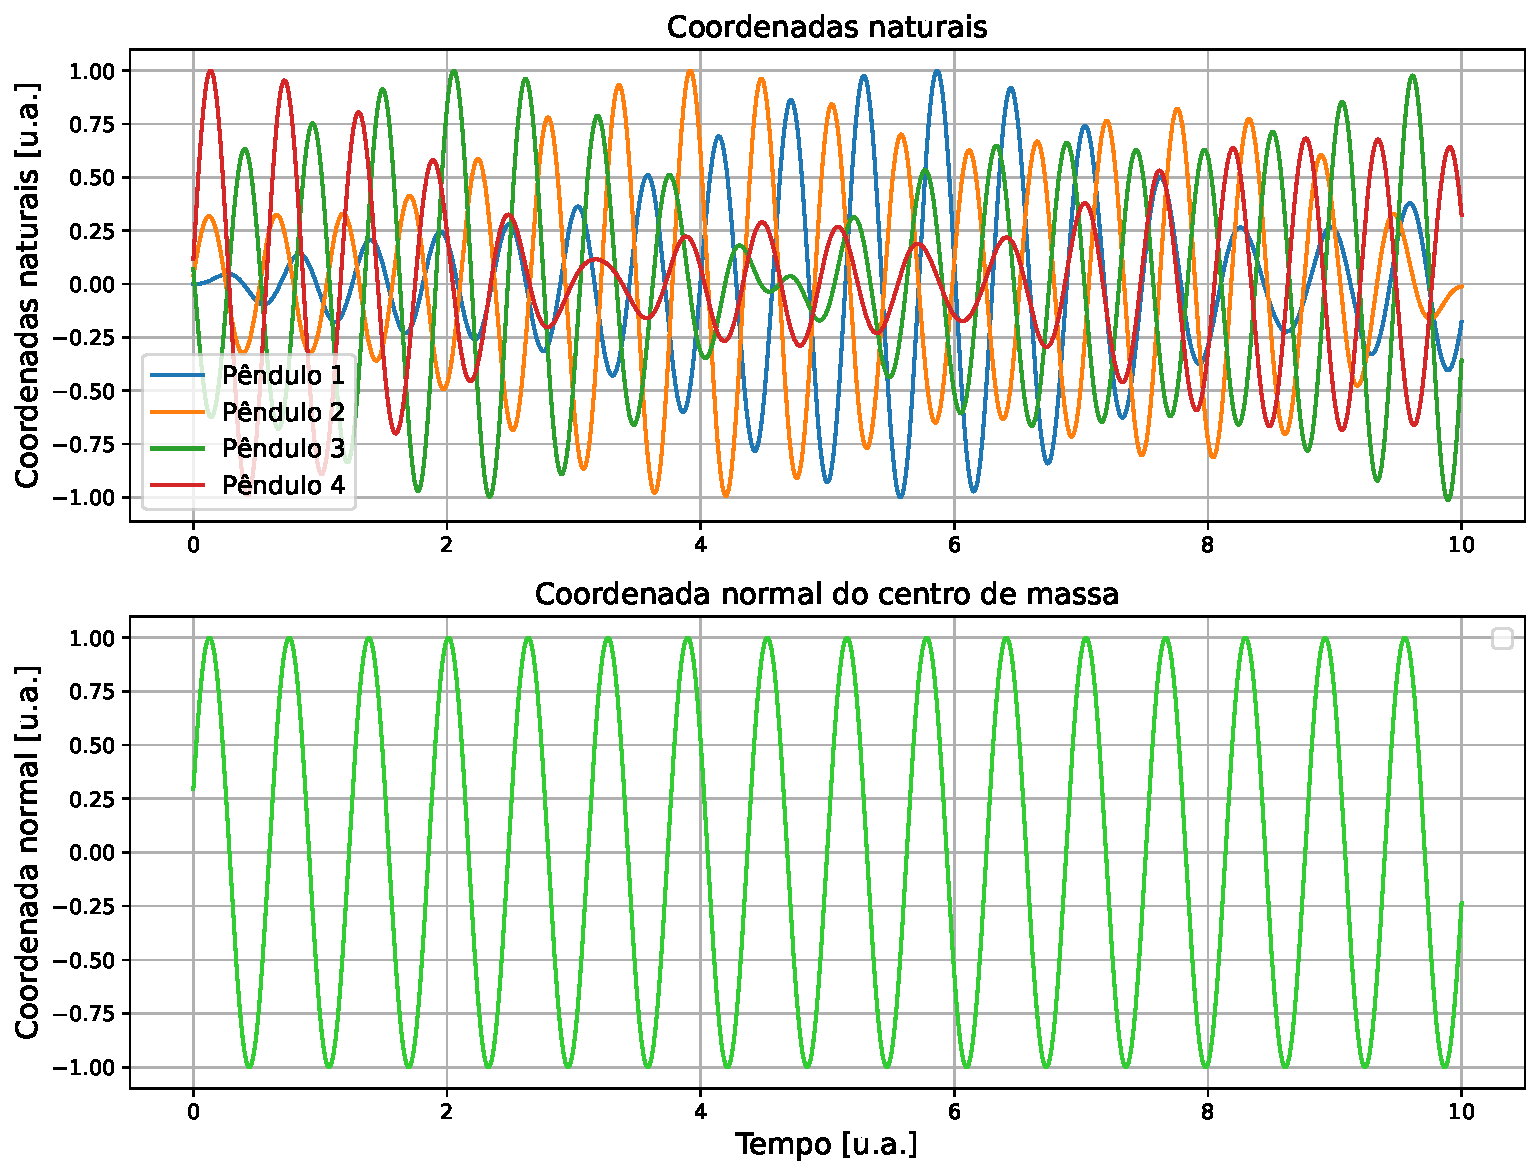
\includegraphics[width=1\linewidth]{graph_coordenadas_pendulos.pdf}
        \caption{Conjuntos de coordenadas naturais e a coordenada normal do centro de massa do sistema para $N=4$ osciladores com condições iniciais diferentes para cada um.
        \label{figura :: coornedas varios pendulos}}
    \end{figure}

    A Figura \ref{figura :: coornedas varios pendulos} mostra os resultados do programa implementado para quatro pêndulos ligados por molas. O modo normal é a coordenada do centro de massa, que é sempre o primeiro dos modos. Futuramente, a perspectiva é implementar esse conjunto de $N$ osciladores ligados por molas.

\newpage
\section{ Conclusões }

    O programa elaborado é capaz de estudar bem o caso dos dois pêndulos acoplados pela mola. Ele é capaz de analisar as soluções para as coordenadas, os perfis do espaço de fase e a energia do sistema. Para o caso de $N>2$ osciladores acoplados, o programa ainda depende de alguns ajustes para determinação dos modos normais, bem como uma aplicação de osciladores ligados por molas com movimento longitudinal e transversal pelas mesmas molas.


\newpage
\nocite{*}
\bibliographystyle{unsrt}
\bibliography{ref.bib}
\addcontentsline{toc}{chapter}{Referências}
\end{document}